\chapter{Introduction}\label{chap:intro}

Understanding the physical processes which have shaped our Universe is the fundamental goal of Astrophysics. A successful theory of the Universe must describe how it evolved from the primordial soup of matter present just after the Big Bang to the variety of galaxy properties we see today. 

The most widely accepted cosmological model is the $\Lambda$-CDM ($\Lambda$- cold dark matter) model which describes a flat Universe made of only $\sim5\%$ baryonic (``normal'') matter, $\sim26\%$ cold dark matter and $\sim69\%$ dark energy \citep{planck16}. In such a Universe, tiny quantum fluctuations in the early Universe grow with time, becoming overdense and laying the foundations for galaxy formation \citep{guth82, hawking82, linde82, starobinsky82}. Given the relatively small fraction of baryonic matter in the Universe, its gravitational contribution to this process is often neglected, greatly simplifying the problem. Structure in simulations is then observed to form hierarchically \citep{press74, gott75, white78, aarseth79, gott79, turner79, efstathiou81, davis85}. At the overdense regions in the early Universe, matter collapses dissipationally under its own gravity forming a dark matter `halo', which then grows through smooth accretion and mergers with other halos to produce the inhomogeneous large scale structure of galaxy filaments, clusters and voids we observe today \citep[see comprehensive review by][]{frenk12}. 

Adding localised baryonic physics into this picture, however, complicates matters. Galaxies are, unfortunately, not just simple smooth dark matter halos; they are thought to start life when baryons cool and condense at the centre of a dark matter halo. Further accretion of matter will cause a gravitational collapse \citep[if angular momentum is present as a result of tidal torques then a rotating gas disc will form][]{fall80, barnes87} and stars will form as hydrogen gas cools and coalesces. From this moment a galaxy will evolve, its shape changing depending on its encounters with other galaxies. 

Today we observe galaxies with a multitude of shapes, or morphologies, across all redshift ranges. \cite{hubble36} classified galaxies based on their shape, producing the widely adopted `tuning fork diagram', now known as the Hubble sequence and shown in Figure~\ref{fig:hubble}. Hubble noticed that galaxies could be broadly categorised as either ellipticals or discs with spiral arms and/or barred structures. He referred to these categories as early-types (placed to the left of his diagram, in keeping with time axis conventions) and late types respectively, because he thought that as galaxies evolved they developed spiral structure. However, as discussed above, cosmological studies have concluded that galaxies start life as a rotating gas disc and so instead, Hubble's diagram is often read from right to left \citep[with some debate over the placement of the S0 galaxies in this picture;][]{kormendy96}. Connecting this picture of pure gas disc galaxies in their infancy with the plethora of galaxy structures we see today, is the focus of this thesis. 

\begin{figure}
\centering{
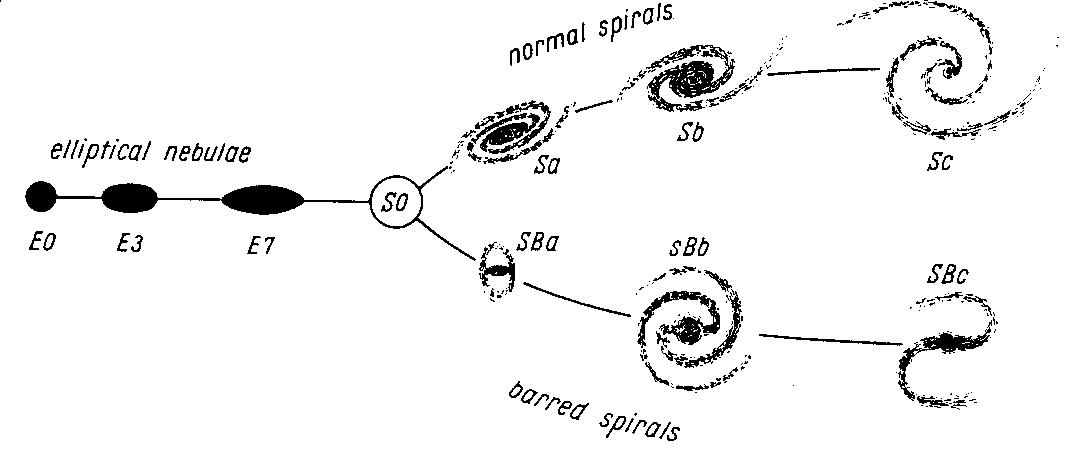
\includegraphics[width=\textwidth]{introduction/hubble.jpeg}}
\caption[The Hubble sequence for morphological classification of galaxies]{The Hubble sequence of galaxy morphology shown on his famous `tuning fork diagram' as published in \cite{hubble36}.}
\label{fig:hubble}
\end{figure}


However, galaxy morphology alone is not enough to characterise a galaxy. The magnitude (used as a proxy for stellar mass), star formation rate (SFR), metallicity (Z) and environment are all crucial to describing a galaxy's current state. By studying these galaxy properties, insights into the processes which govern galaxy evolution can be gained.

Large scale surveys of galaxies first revealed a bimodality in the optical colour-magnitude diagram (CMD) of galaxies revealing two distinct populations (see Figure~\ref{fig:cmdbaldry}); one at relatively low mass with blue optical colours and another at relatively high mass with red optical colours \citep{Baldry04, Baldry06, Willmer06, ball08, Brammer09}. These populations were dubbed the `blue cloud' and `red sequence' respectively \citep{Chester64, bower92, Bell04, Driver06, Faber07}.  The sparsely populated colour space between these two populations was dubbed the  `green valley'.

\begin{figure}[t]
\centering{
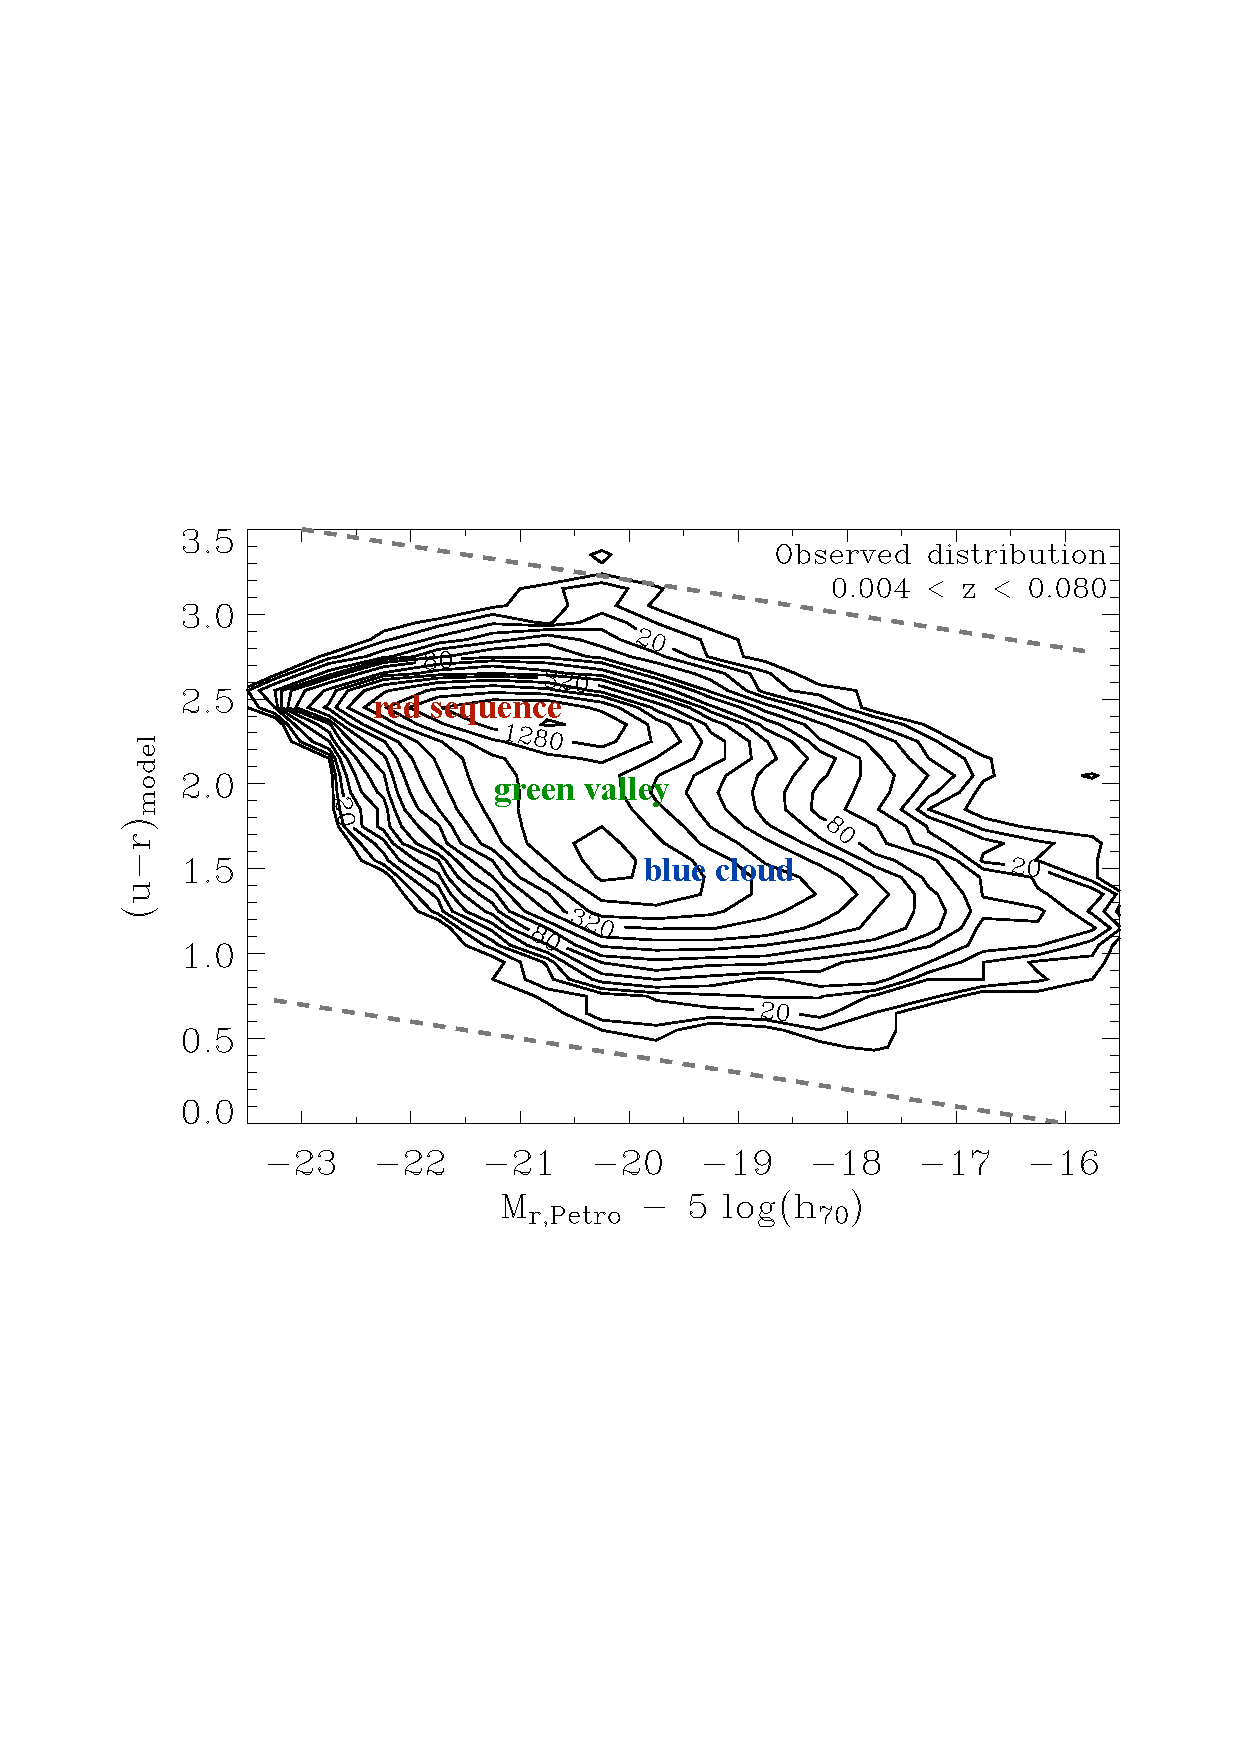
\includegraphics[width=\textwidth]{introduction/cmd.pdf}}
\caption[Galaxy Colour Magnitude Diagram from \cite{Baldry04}]{The galaxy colour magnitude diagram as observed by \cite{Baldry04}. The figure has been adapted from Figure 1 in \citeauthor{Baldry04} and annotated to show the locations of the red sequence and blue cloud. A lower magnitude corresponds to a higher mass and a large $u-r$ value corresponds to a redder colour.}
\label{fig:cmdbaldry}
\end{figure}


The majority of disc galaxies were found in the blue cloud and the majority of ellipticals on the red sequence, with colour often used as a proxy for morphology. The Galaxy Zoo project \citep{lintott08, Lintott11}, which produced morphological classifications for a million galaxies, helped to confirm that this colour bimodality is not entirely morphology driven \citep{Strat01, Salim07, Sch07, CHV08, Bamford09, Skibba09}, detecting larger numbers of spiral galaxies in the red sequence \citep{masters10c} and elliptical galaxies in the blue cloud \citep{Sch09} than had previously been observed. A change in colour therefore doesn't always coincide with a change in morphology. 

Large galaxy surveys also revealed that star forming galaxies are observed to lie on a well defined `star forming sequence' (SFS) in the stellar mass vs. star formation rate (SFR) plane \citep{brinchmann04, Salim07, daddi07}. The majority of blue cloud galaxies are found to lie on this SFS with the majority of the red sequence lying well below it with very low SFRs. The green valley, which lies between the red sequence and blue cloud, is therefore assumed to contain galaxies which have recently undergone a suppression of star formation \citep[SF;][]{Salim07}. This suppression of SF and subsequent transition of a galaxy from blue cloud to red sequence must therefore also be intrinsically tied with a possible change in morphology from a disc galaxy to an elliptical galaxy. This is entirely possible in hierarchical structure formation through mergers of galaxies.

The discovery of the fundamental plane \citep{dressler87, djorgovski87}, wherein the stellar velocity dispersion is correlated with the luminosity and effective radius of an elliptical, further constrained the mechanisms responsible for galaxy formation. The fundamental plane can be reproduced in simulations of major mergers \citep{bekki98, nipoti03, boylan05, robertson06, hilz12, taranu15}, lending support to the theory of hierarchical structure formation.

Further evidence for hierarchical structure formation is that galaxies are often found huddled together in groups \citep{zwicky38, zwicky52, abell58}, all sharing one large dark matter halo (groups with 100 or more galaxies are referred to as clusters \citealt{bower04}). Conversely some galaxies are found isolated from others in less dense environments (often referred to as the field), either because they are fossil groups \citep[where all members have eventually merged][]{ponman94, jones00, jones03} or have truly been isolated for their entire lifetimes. This environmental density is found to be correlated not only with morphology \citep[][and see Figure~\ref{fig:dressler}]{dressler80, smail97, poggianti99, postman05, Bamford09}, but also colour \citep{butcher78, pimbblet02}, quenched galaxy fraction \citep{kauffmann03, Baldry06, peng12, darvish16} and SFR \citep{gomez03} suggesting that the environment may drive this transition from blue cloud to red sequence through increasing the likelihood of galaxy mergers. 

\begin{figure}[t]
\centering{
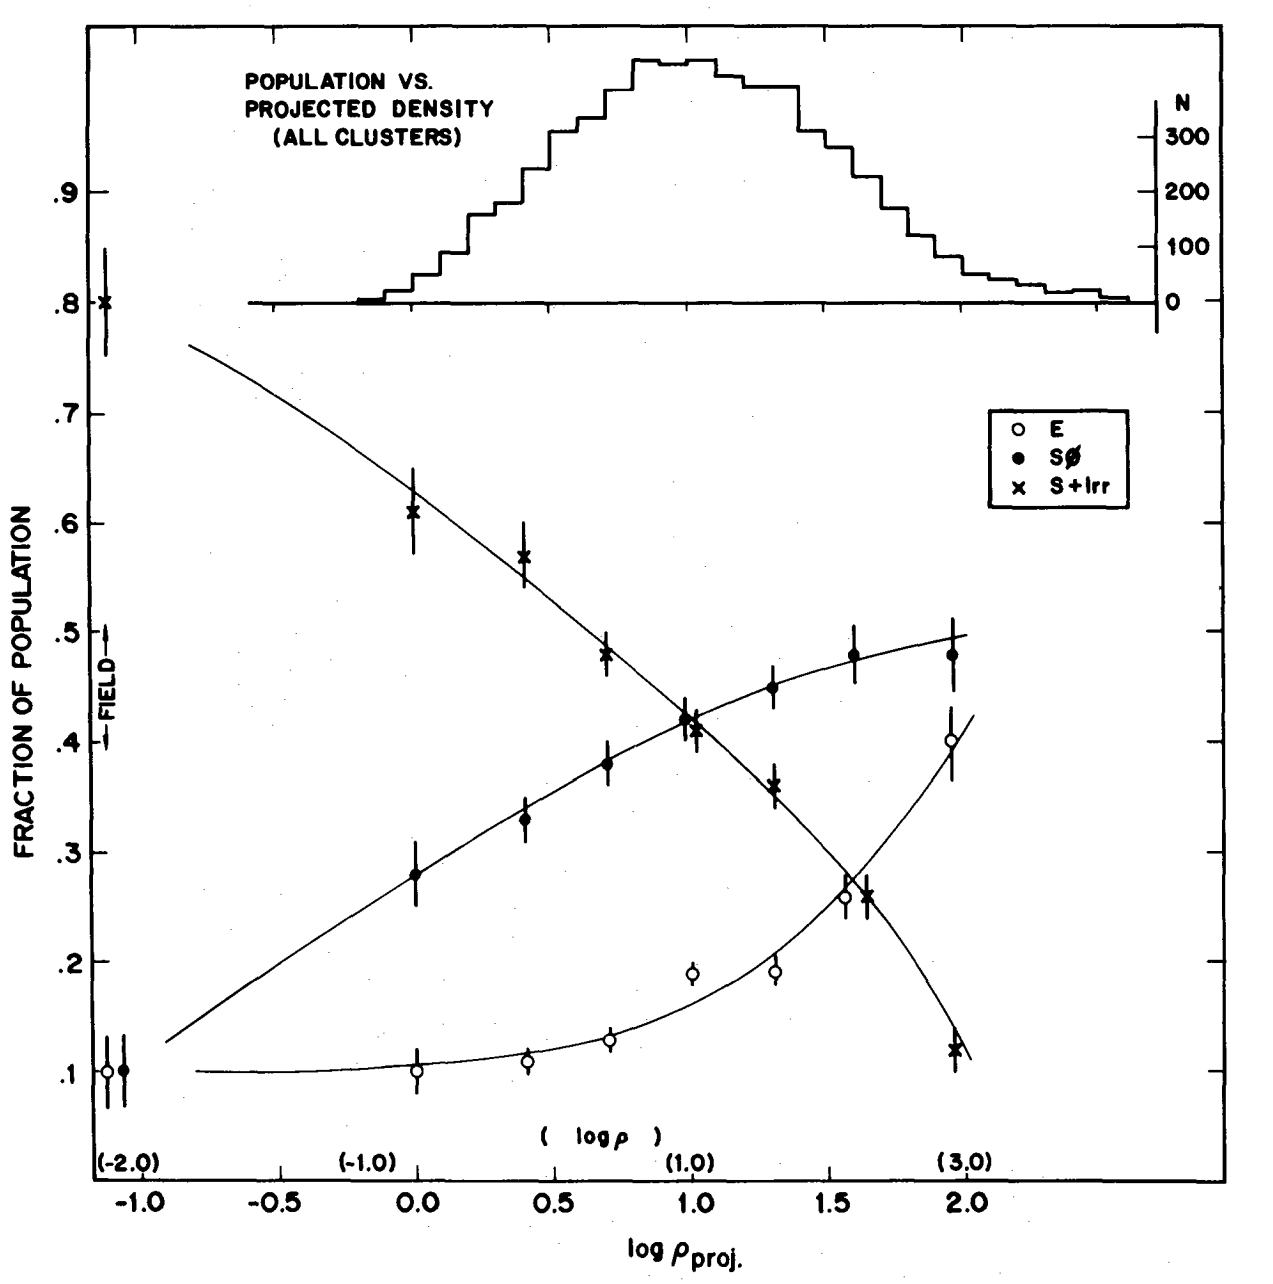
\includegraphics[width=0.8\textwidth]{introduction/dressler.png}}
\caption[Morphology Density relation from Figure 4 of \cite{dressler80}]{The morphology-density relation from Figure 4 of \cite{dressler80} showing how the fraction of ellipticals (E) increases with increasing environmental density and the fraction of spirals (S + Irr) decreases.}
\label{fig:dressler}
\end{figure}

However, within the framework of hierarchical structure formation, the observed mass-metallicity relation \citep{tremonti04} cannot be reproduced. This relationship describes how higher mass galaxies have higher metal contents. Simulations have shown that this phenomenon cannot be reproduced by the merging of galaxies alone, since mergers dilute the metallicity \citep{pipino08,rupke10, montuori10, torrey12}. This is also supported by observations showing that metallicities in galaxy pairs are suppressed by $\sim0.05~\rm{dex}$ \citep{ellison08, michel08, scudder12}. There must therefore be processes other than mergers occurring which are responsible for the colours, SFRs, masses, metallicities and morphologies of galaxies observed. 

Further insight has also recently been revealed by the number of integral field unit (IFU) surveys which have come online in the past couple of years. These include the SAURON instrument \citep{bacon01}, the completed $\rm{ATLAS}^{\rm{3D}}$ survey \citep{cappellari11} which targeted a small sample of 260 early-type galaxies, and the larger, ongoing surveys of MaNGA \citep{bundy15}, SAMI \citep{croom12} and CALIFA \citep{sanchez12}. Upon completion at the end of the decade, these surveys are expected to revolutionise the field of galaxy evolution, providing spatially resolved maps of SF indicators for over $10,000$ galaxies.

Even with the higher resolution data forthcoming, there is still value in studying galaxies which have just left the SFS, to reveal the mechanisms governing galaxy evolution, including both the suppression of SF and the possible transformation of galaxy structure. Green valley galaxies have long been thought of as the `crossroads' of galaxy evolution, a transition population between the star forming blue cloud and the quiescent red sequence. \citet{Bell04} were the first to recognise that green valley galaxies may be a transitional population between the blue cloud and red sequence. \citet{Wyder07} confirmed that galaxy bimodality also appears in NUV-optical colour space, with \citet{Schim07} investigating the morphological dependence in this parameter space and \citet{Martin07} using it to constrain the flux of galaxies transitioning through the green valley. \citet{Faber07} suggested that the build up of the red sequence has to occur via a mixture of suppression of star formation of galaxies in the blue cloud and mergers on the red sequence, which was confirmed by \citet{Mendez11} who showed that mergers alone are not responsible for the transition from the blue cloud. This transition was theorised to occur on rapid timescales, otherwise there would be an accumulation of galaxies residing in the green valley \citep{Gonc12}; however \citet{schawinski14} concluded that this was only true for elliptical galaxies, with disc galaxies transitioning much more slowly. The morphological dependence and causes of this transition are therefore still the cause of much debate. 


This thesis will focus on studying this transition and the mechanisms responsible. I will refer to the suppression of a galaxy's SFR as \emph{quenching} and processes which can cause this suppression as \emph{quenching mechanisms}. 

\section{Possible quenching mechanisms}\label{sec:quenchmech}

There are many theorised mechanisms which can cause quenching. They are often referred to as either \emph{internal} mechanisms (caused by the galaxy's \emph{nature}) or \emph{external} mechanisms (caused by the way the galaxy is \emph{nurtured}). The properties of a galaxy and its environment are often thought to control which mechanisms will affect a galaxy throughout its lifetime and subsequently affect the morphology. 

%There have been many previous theories for the initial triggers of these quenching mechanisms, including negative feedback from AGN \citep{diMatteo05, Martin07, Nandra07, Sch07}, mergers \citep{Darg10a, Cheung12, Barro13}, supernovae winds \citep{MFB12}, cluster interactions \citep{Coil08, Mendez11, Fang13} and secular evolution \citep{masters10c, masters11a, Mendez11}. By investigating the \emph{amount} of quenching that has occurred in the blue cloud, green valley and red sequence; and by comparing the amount across these three populations, I can apply some constraints to these theories. 
\subsection{Internal Quenching Mechanisms}\label{sec:intquench}

\subsubsection{AGN feedback as a quenching mechanism}\label{sec:agnquench}

An active galactic nucleus (AGN) is an actively growing supermassive black hole in the centre of a galaxy. There are many observed spectral classes of AGN which are explained by the viewing angle in the theory of unification \citep[see review by][]{netzer15}. The basic structure of an AGN consists of an accretion disc of cold material which is formed around the black hole as the material inspirals and is pulled into a single orbital plane by the force of gravity. The friction built up by the rotating gas causes the accretion disc to heat up and emit large amounts of energy in the form of X-rays. The accretion disc is also surrounded by a broad line region and an absorption region (often referred to as the torus) which can both absorb and re-emit the emitted light from the accretion disc (for a diagram depicting AGN structure see \citealt{beckmann12}). Type 2 Seyfert AGN are those which are viewed approximately edge on to their accretion disc and so have the majority of their emitted light absorbed by the torus. Some light is scattered off the surrounding gas clouds, resulting in the detection of broadened spectral emission lines. Type 1 Seyfert AGN however are those which are viewed perpendicular to their accretion disk and so are unobscured by the torus; light from both the accretion disc and/or emitted radiation jets can be observed. 

% \begin{figure}[t]
% \centering{
% 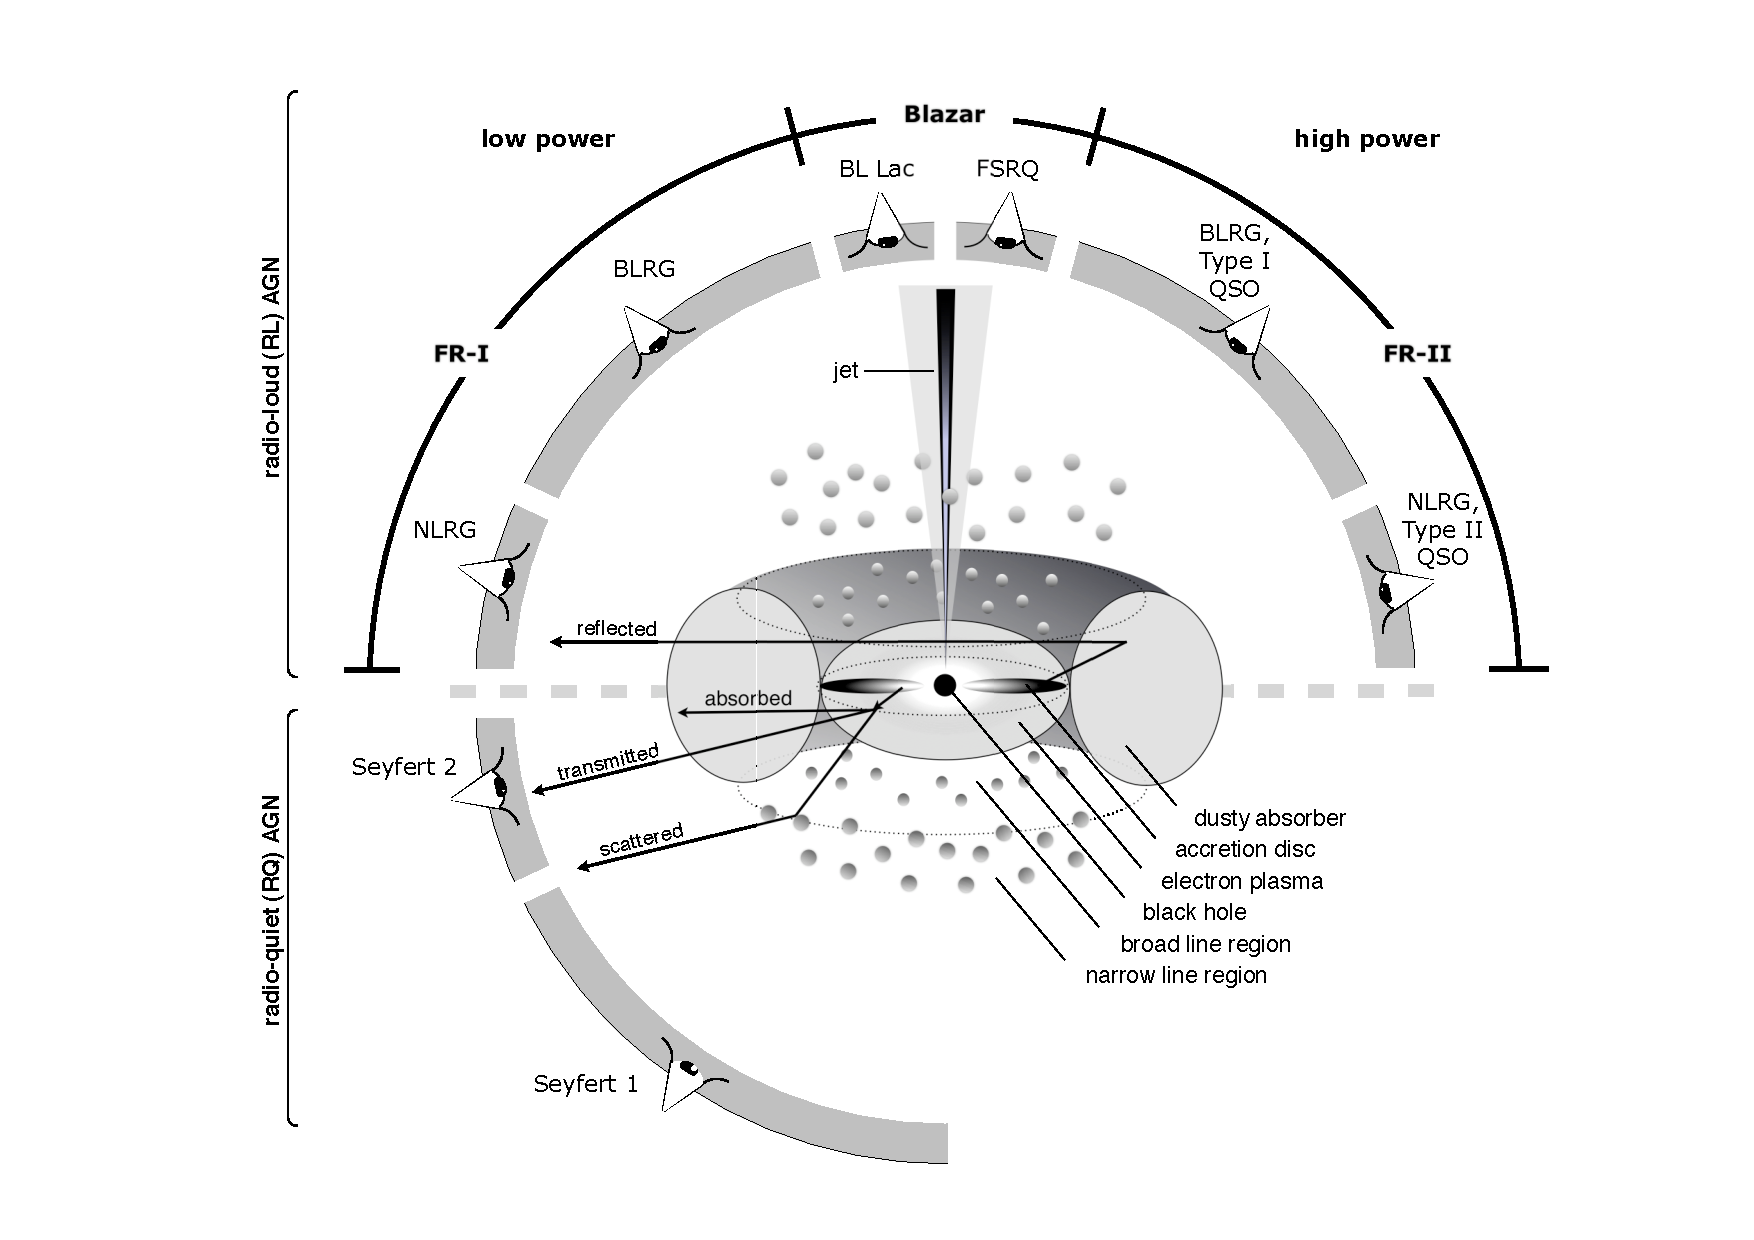
\includegraphics[width=0.9\textwidth]{introduction/agn_unification.pdf}}
% \caption[Illustration of the structure of an AGN from \cite{beckmann12}]{Cartoon of the structure of an AGN including the accretion disc, dusty absorber (often referred to as the obscuring torus) \& output jet, in the context of viewing angle for various spectral classes of observed AGN.}
% \label{fig:agntorus}
% \end{figure}

There are tight correlations between properties of galaxies, such as the bulge mass, total stellar mass \& stellar velocity dispersion, and the black hole mass \citep{magorrian98, marconi03, haringrix04}. This implies a co-evolution between the black hole and its host galaxy therefore suggesting that changes in the SFR and structure of a galaxy could also be tied to black hole activity. 

If we consider a `back of the envelope' calculation of the ratio between the total energy of the black hole and the binding energy of the galaxy, we can determine if output from the black hole will be able to have a significant effect on its host galaxy \citep[see p.649 of][]{mo10}. The total energy output by a black hole in its lifetime can be expressed as $E_{BH} = \overline{\epsilon}M_{BH}c^2$, where $\overline{\epsilon}$ is the mean efficiency of the black hole of mass $M_{BH}$. The galaxy binding energy can be approximated as $E_{gal} \approx M_{*}\sigma^2$, where $M_{*}$ is the stellar mass of the galaxy with stellar velocity dispersion $\sigma$. Taking the average values of $M_{BH} \sim 10^{8.0}~\rm{M}_{\odot}$,~$M_{*} \sim 10^{10.8}~\rm{M}_{\odot}$ and $\sigma \sim 200~\rm{km}~\rm{s}^{-1}$, of the 30 galaxies observed by \citet{haringrix04}, we can estimate the ratio $E_{BH}/E_{gal} \sim \overline{\epsilon} 10^3$. If the efficiency of the black hole is $\sim15\%$ \citep{elvis02}, the energy of the black hole can easily surpass the binding energy of its galaxy, suggesting that a black hole can indeed impact its host. This is thought to occur via AGN feedback where the output of energetic material and radiation from the black hole is theorised to either heat or expel the gas needed for SF in a galaxy, causing a quench. Energy from a black hole is observed to be ejected in narrow, collimated jets of material out of the plane of a galaxy \citep[see review by][]{homan12}, but for AGN feedback to be effective these jets would somehow need to impact the gas in the entire galaxy. 

\begin{figure}[t]
\centering{
\includegraphics[width=0.8\textwidth]{introduction/silk_mamon_LF.pdf}}
\caption[Illustration of the mismatch between theoretical and observed luminosity function from \cite{silk12}]{Cartoon of the role of feedback in modifying the observed luminosity function of galaxies with respect to theoretical predictions. Supernova winds are thought to be responsible at the low mass end, with AGN feedback responsible at the high mass end. Figure 1 in \cite{silk12}.}
\label{fig:lumfuncpic}
\end{figure}

AGN feedback was first suggested as a mechanism for regulating star formation due to the results of simulations wherein galaxies could grow to unrealistic stellar masses \citep{silk98, Bower06, Croton06, somerville08}. Without a prescription for the effects of AGN feedback, the shape of the galaxy luminosity function could therefore not be matched at the high luminosity end \citep{baugh98, baugh05, kauffmann99a, kauffmann99b, somerville01, kitzbichler06}. A similar problem was also encountered at the low end of the luminosity function, which was rectified by the inclusion of the effects of supernova wind feedback \citep{dekel86, powell11}. This is illustrated in Figure~\ref{fig:lumfuncpic} taken from \cite{silk12}. 

Indirect observational evidence has now been found for both positive and negative feedback in various systems (see the comprehensive review from \citealt{fabian12}). The strongest being the indirect evidence that the largest AGN fraction is found in the green valley \citep{cowie08, Hickox09, schawinski10a}, suggesting a link between AGN activity and the process which moves a galaxy from the blue cloud to the red sequence. However, concrete statistical evidence for the effect of AGN feedback on the host galaxy population has so far been elusive.


\subsubsection{Mass quenching}\label{sec:massquench}

Mass quenching is defined by \citet{peng10, peng12} as any quenching mechanism acting independently of a galaxy's environment, but not of its mass. However, there is still much debate over the exact mechanism which is the cause of such a quench. \citet{darvish16} suggest that non-AGN driven feedback mechanisms (for example supernova feedback) are responsible for the correlation observed between the mass quenching efficiency and SFR in \citet{peng10}. However, \citet{gabor15} suggest that this is driven by ``halo quenching processes'' whereby the inflow of cool gas from the galaxy halo is either cut off or hindered from cooling at $M_{halo} > 10^{12}~\rm{M}_{\odot}$ \citep{birnboim03, dekel06}. If this happens, a galaxy uses up the rest of its available gas for star formation via the Kennicutt-Schmidt law \citep{schmidt59, kennicutt98} and consequently grows in mass.

In the rest of this thesis, I refer to mass quenching as a cut off of gas inflow, resulting in a gradual consumption of gas in star formation. This definition of mass quenching is thought to be a dominant mechanism for isolated galaxies in the field \citep{kormendy04}. However, it is also thought that as a galaxy infalls in to a group or cluster over long timescales, gas reservoirs can also be depleted via a mass quenching process \citep{peng12}. 

 
\subsubsection{Morphological quenching}\label{sec:moprhquench}

Morphological quenching is the process by which the internal structure of a galaxy can have a negative impact on its own SFR\footnote{Essentially shooting itself in the foot.}. This can happen in one of two ways, either by preventing star formations from occurring or by increasing the rate of consumption of gas for star formation. The former is theorised to be caused by bulges \citep{bluck14} whereby the large gravitational potential of the bulge prevents the disc from collapsing and forming stars \citep{Fang13}. 

The latter mechanism is theorised to occur in galaxies hosting bars; the bar funnels gas to the centre of the galaxy \citep{athanassoula92a} where gas is exhausted by star formation effectively quenching the galaxy \citep{zurita04, sheth05}. This process is thought to be responsible for large numbers of red spirals and supported by observations of increasing bar fraction with red colours \citep{masters11a}. Recent observational evidence from \cite{hart16} also suggests that spiral structure can also cause morphological quenching. \citeauthor{hart16} propose that many armed spiral structures can trigger galaxy wide starbursts thereby rapidly using up gas for future star formation; similarly two armed spirals are observed with redder colours, suggesting that this spiral phase is much longer lived and may funnel gas into the centre of the galaxy to be exhausted in star formation over longer timescales.  
  
\subsection{External Quenching Mechanisms}\label{sec:extquench}
  
\subsubsection{Mergers as a quenching mechanism}\label{sec:mergersquench}

Major mergers have been intrinsically linked to the formation of elliptical galaxies since \citet{toomre72} showed this was possible with a simulation of the merger of two equal mass disc galaxies. Since $\Lambda$-CDM relies on the idea of hierarchical structure formation through the merger of dark matter halos for its description of galaxy formation, it also follows that galaxy evolution should be further influenced by mergers. 

The hypothesis is as follows: when two galaxies merge, the influx of cold gas funnelled by the forces in the interaction often results in energetic starbursts \citep{mihos94, mihos96, hopkins06d, hopkins08a, hopkins08b, snyder11, hayward14, sparre16}, which can exhaust the gas required for star formation, effectively quenching the post-merger remnant. This remnant galaxy will also have formed a dynamically hot bulge through the dissipation of angular momentum in the merger \citep{toomre77, walker96, kormendy04, hopkins11c, martig12}. The mass ratio of the two galaxies merging is thought to affect the size of the bulge that is formed in the remnant \citep{cox08, hopkins09c, tonini16}, with the most massive major mergers with a 1:1 mass ratio producing fully elliptical galaxies \citep{toomre72, barnes96, mihos96, kauffmann96, pontzen16}.

Such a scenario is also intrinsically linked to the triggering of an AGN due to the influx of gas in the merger which can fuel the black hole accretion \citep{sanders88, dimatteo05, hopkins09a, treister12}. Many studies have therefore focussed on investigating the growth of black holes due to mergers \citep[e.g.][]{veilleux02, bellovary13, ellison13, medling15, gabor16}. Simulations of mergers with AGN have lead many to believe that a merger which triggers both a starburst and an AGN can quench a galaxy in extremely rapid timescales \citep{springel05b, bell06}. Recent simulations have also suggested that feedback from the triggered AGN (see Section \ref{sec:agnquench}) is necessary to fully remove (or heat) all the available gas, otherwise the SFR will recover back to the SFS post-merger \citep{pontzen16, sparre16}. 

Mergers also have a clear environmental dependence, as they are more likely to occur in denser environments. However, their effects must be separated from those quenching mechanisms driven solely by the properties of the galaxy environment. 

\subsubsection{Environment driven quenching}\label{sec:envquench}

The environment of a galaxy has long been considered a key  \emph{nurturing} aspect of galaxy evolution. Correlations of galaxy morphology \citep{dressler80, smail97, poggianti99, postman05, Bamford09}, colour \citep{butcher78, pimbblet02} and the quenched galaxy fraction \citep{kauffmann03, Baldry06, peng12, darvish16} with the environmental density all suggest that the environment is in some way responsible for the build up of the red sequence through quenching. 

The proposed quenching mechanisms under the umbrella of environmental quenching are numerous and varied. Together with the typical gravitational galaxy-galaxy interactions \citep{moore96} which are expected to be more frequent in a dense environment, environmental quenching also includes hydrodynamic interactions occurring between the cold interstellar medium (ISM) of the in-falling galaxy and the hot intergalactic medium (IGM) of the group or cluster. Such hydrodynamic interactions include ram pressure stripping \citep{gunngott72}, viscous stripping \citep{nulsen82}, and thermal evaporation \citep[a rapid rise in temperature of the ISM due to contact with the IGM;][]{cowie77}. Another such process is starvation \citep[also called strangulation;][]{larson80} which can remove the outer galaxy halo, thus cutting off the star formation gas supply to a galaxy. Preprocessing occurs when all of the above mechanisms take place in a group of galaxies which then merges with a larger group or cluster \citep{dressler04}. 

The most likely (and therefore the most studied) candidate mechanism for the cause of the environmental density-morphology and SFR relations is ram pressure stripping \citep[RPS;][]{abadi99, poggianti99}. However, there has been mounting evidence that RPS can only strip a galaxy of $40-60\%$ of its gas supply \citep{fillingham16} and so may not be as effective a quenching mechanism as first thought \citep{emerick16}. Therefore investigations of other environmentally driven quenching mechanisms, such as strangulation \citep{peng15, hahn16, maier16, paccagnella16, roberts16, vandevoort16} and harassment \citep[high speed galaxy `fly-by' gravitational interactions][]{bialas15, smith15b} are having a recent resurgence. 

\section{Using star formation histories to investigate quenching}\label{sec:invquench}

% previous work
% using SFHs
% the benefits of SPSs

In order to understand how a galaxy is quenched, the star formation history (SFH) is often modelled. This approach requires the inference of the global SFH of a galaxy from its current stellar population. While it is possible to observe resolved stellar populations for nearby galaxies with the \emph{Hubble Space Telescope} (HST) in order to pinpoint the main sequence turn off (an indicator of the age of a stellar population) on the Hertzsprung Russell diagram, this is not possible in more distant galaxies. Instead, reliance is placed upon the correlation between the integrated total light of a galaxy and its SFH \citep{searle73}. Adopting a global SFH for a galaxy is a big assumption, especially since recent IFU studies have shown that bulges and discs have vastly different SFHs \citep[see for example][]{johnston16}. However, these differences will smear out across the integrated light of a galaxy and so inferring the SFH in this way will give an estimate of the average global SFH of the galaxy. This is still useful information, especially when investigating the average quenching history of a large population of galaxies.

Many studies have employed this technique using either photometric broadband colours or spectral data as indicators of the integrated SFH \citep[for example][]{deJong96, madau98, davies01, kauffmann03, dressler04, macarthur04, Martin07, perez11, sanchez11, mcdermid15}. However, this technique is sensitive to the degeneracies between age and metallicity \citep{worthey94} as well as the effects of dust \citep{ganda09, pastrav13} on the integrated light. 

The turn of the millennium therefore saw the development of full spectral energy density (SED) fitting codes to infer the SFH (without having to make any prior assumptions on its form) such as \textsc{moped} \citep{heavens00}, \textsc{starlight} \citep{cidfernandes05}, \textsc{vespa} \citep{tojeiro07}, and more recently \textsc{firefly} \citep{wilkinson15}. In the absence of spectral data however, broadband colours are still effective at inferring the global SFHs of galaxies, especially when wavebands across the spectrum, such as ultra-violet, optical and infrared colours are used simultaneously \citep{madau98}. 

This method is achieved by modelling the observed SED of a galaxy using a combination of SEDs of simple stellar populations (SSP) at various ages. SSPs assume that stars are coeval and form with the same metallicity and comprehensive knowledge of stellar evolutionary tracks and initial mass functions \citep[IMF;][]{salpeter55, chabrier03} are therefore needed to calculate the spectrum of a SSP at a given age \citep{chen10, kriek10}. Luckily, some astronomers have made the study of these SSPs their life's work \citep[for example]{BC03, Maraston05, vazquez05, CGW09}, therefore once an IMF and a SFH function have been assumed, the SED of a model galaxy can be predicted at any point in its history \citep{chen10}. This technique also assumes a universal IMF, which recent studies have shown may not be appropriate \citep{vandokkum08, conroy12, cappellari12, smithr15}. Whilst the choice of an IMF and metallicity of a SSP will affect the output SED \citep{CGW09, kriek10}, the choice of the functional form of the SFH will have the greatest impact. 

Many possible forms for global galaxy SFHs have been assumed in previous studies, including an exponential decline \citep{tinsley72, gavazzi02, weiner06, Martin07, noeske07, kriek10,  schawinski14, hart16}, the extended (or delayed) exponential model \citep{gavazzi02, oemler13, simha14}, a Gaussian distribution \citep{feuillet16} or a log normal distribution \citep{gladders13, abramson16}. The studies of \cite{lee10}, \cite{boquien14} and \cite{smith15} have shown that these SFHs don't accurately characterise the detailed SFH of a galaxy, as they generalise the localised bursts of star formation across a galaxy's lifetime into a global SFH. In an investigation of the SFH of a single galaxy these forms of the SFH are therefore not appropriate, however, when studying the general quenching histories of a large population of galaxies these functional forms are still appropriate. They still allow for insight to be gained on the complex processes responsible for the galaxy properties observed across the population by allowing the quenching history to be described by just $2$ parameters. 

In this thesis I will assume an exponentially declining SFH, following the work of \cite{schawinski14}, for galaxies with morphological classifications from Galaxy Zoo. Employing Bayesian methods, I will use optical and NUV photometry to infer the dependence of quenching histories on the morphology across the colour magnitude diagram. I will also investigate the quenching histories of galaxies that host AGN and those in dense environments to help constrain the quenching mechanisms responsible for galaxy evolution.

\section{Data}\label{sec:data}

In the following section I describe the data sources for the optical \& NUV colours and morphologies used throughout this study.

\subsection{Sloan Digital Sky Survey}\label{sec:sdssintro}

The Sloan Digital Sky Survey (SDSS; \citealt{york00}) is an optical imaging and spectroscopic survey of $8,000$ square degrees of sky, which was completed using a $2.5\rm{m}$ telescope at Apache Point Observatory in New Mexico, USA. SDSS Data Release 8 \citep{aihara11} provided publicly available optical magnitudes across $5$ broadband filters, $ugriz$, for over 1 million galaxies in the `main galaxy' sample. Here I utilise the Petrosian magnitude, {\tt petroMag}, values for the $u$ ($3,543\rm{\AA}$) and $r$ ($6,231\rm{\AA}$) wavebands provided by the SDSS pipeline. Spectral data is available for a significant proportion of the SDSS main galaxy sample but the spectral fibre is a set size. Therefore across a population of galaxies the fibre will cover varying radii depending on the distance and size of a galaxy. Therefore the usual spectral star formation indicators cannot be utilised in this study as they will over- or under-estimate the global average SFR of a galaxy. 

Magnitudes are corrected for galactic extinction \citep{Oh11} by applying the \citet{Cardelli89} law, giving a typical correction of $u-r \sim 0.05$. K-corrections are also adopted to $z=0.0$ and absolute magnitudes obtained from the NYU-VAGC \citep{Blanton05, padmanabhan08, blanton07}, giving a typical $u-r$ correction of $\sim 0.15$ mag. The change in the $u-r$ colour due to both corrections therefore ranges from $\Delta (u-r) \sim 0.2$ at low redshift, increasing up to $\Delta (u-r) \sim 1.0$ at $z \sim 0.25$, which is consistent with the expected k-corrections shown in Figure 15 of \citet{blanton07}. These corrections were calculated by \citet{Bamford09} for a subset of galaxies in the SDSS survey. These corrections are a crucial aspect of this work since a $\Delta (u-r) \sim 1.0$ can cause a galaxy to change whether it is classed as blue cloud, green valley or red sequence.

Star formation rates and stellar masses, where available, were obtained from the MPA-JHU catalogue \citep{kauffmann03, brinchmann04}. These SFRs are derived from emission lines using the method of \cite{charlot01}. All SFRs are corrected for aperture size by fitting to the photometry outside the fibre with stochastic models as in \cite{Salim07}. SFRs for non star forming galaxies and AGN were derived indirectly using the $4,000\rm{\AA}$ break. For those galaxies with emission lines with low signal-to-noise ratio, the SFR was estimated indirectly using a conversion factor likelihood distribution between the luminosity of the H$\alpha$ Balmer emission line and the SFR. Masses are obtained from fits to the photometry with a large grid of SFHs produced using the \cite{BC03} models. In this thesis these values are obtained for interest to compare samples; they are never used to infer the SFHs of galaxies due to the circular nature of the modelling used to derive these values and infer the SFHs. I use the average values of \textsc{avg sfr} and \textsc{avg mass} from the inferred likelihood distributions for each galaxy.

\subsection{Galaxy Evolution Explorer}\label{sec:galexintro}

The \emph{Galaxy Evolution Explorer} (GALEX; \citealt{Martin05}) is an ultra-violet space based telescope which images galaxies simultaneously in two broadband filters: both the far ultra-violet (FUV) with an effective wavelength of $1,516\rm{\AA}$ and in the NUV with an effective wavelength of $2,267\rm{\AA}$. Sources detected with GALEX were matched with a search radius of $1''$ to the SDSS data in right ascension and declination. The {\tt auto} magnitudes provided by the GALEX pipeline are used in this study (for a discussion of aperture bias between different surveys see \citealt{hill11}). All magnitudes are k-corrected and extinction corrected as described in Section~\ref{sec:sdssintro}.

\subsection{Galaxy Zoo}\label{sec:GZ}

Galaxy Zoo (GZ) is a citizen science project enlisting the help of thousands of members of the public to voluntarily classify galaxy images online\footnote{\url{http://galaxyzoo.org}}. The first version of GZ classified just under 1 million SDSS galaxy images as either ellipticals, spirals or mergers within approximately 6 months of launch \citep{lintott08, Lintott11}. In the second version, GZ2 \citep{GZ2}, volunteers were asked to make more detailed morphological classifications of $304, 022$ images from the SDSS DR8 (a subset of those classified in the first Galaxy Zoo; GZ1). These images were all classified by \emph{at least} 17 independent volunteers, with the mean number of classifications standing at $\sim42$. GZ is now in its tenth year of classifying and its fifth incarnation, after classifying images from Hubble Space Telescope Legacy surveys in GZ:Hubble \citep{willett16} and the CANDELS survey galaxies in GZ:CANDELS \citep{simmons16}. At the time of writing, images from the DeCALS\footnote{\url{http://legacysurvey.org/}} survey and Illustris simulation \citep{vogelsberger14, genel14} are being classified by volunteers. 

\begin{figure}
\centering{
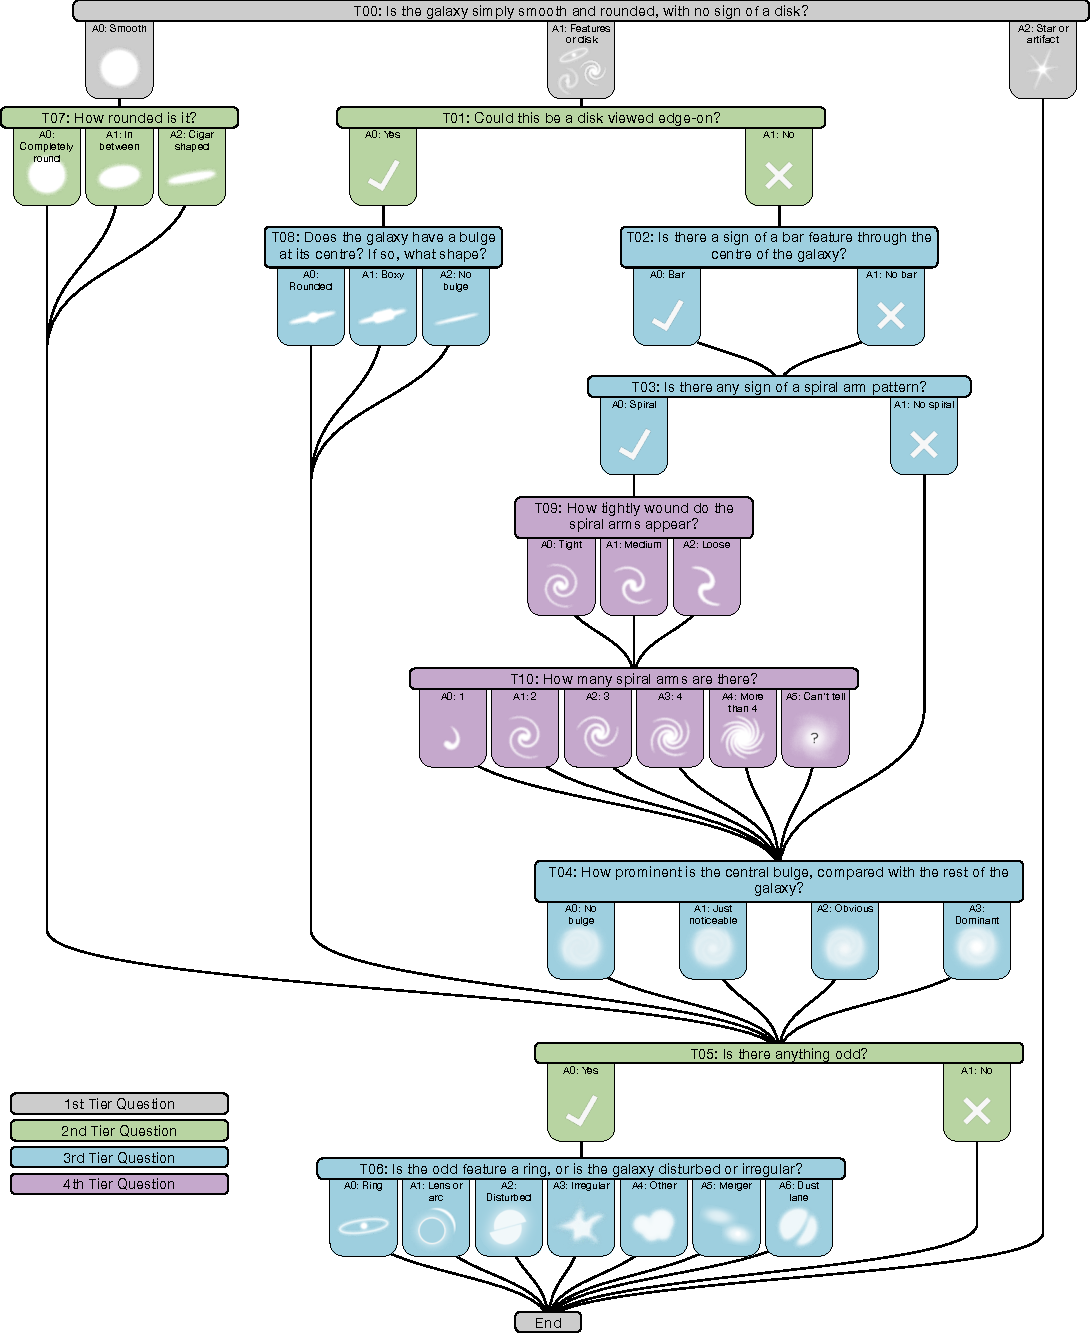
\includegraphics[width=\textwidth]{introduction/gz2_tree.pdf}}
\caption[GZ2 classification decision tree]{Flowchart of the classification tree for GZ2, beginning at the top with Task 0. Tasks are colour-coded by their relative depths in the decision tree with tasks in green, blue and purple respectively one, two or three steps below branching points in the decision tree.}
\label{fig:gztree}
\end{figure}

From GZ2 onwards, all projects have collected classification data via a multi-step decision tree, shown in Figure~\ref{fig:gztree}.  Each individual step in a tree is a \emph{task}, which consists of a \emph{question} with a finite number of possible \emph{answers}. The selection of an answer is called the volunteer's \emph{vote}. The first task of GZ2 asks volunteers to choose whether a galaxy is mostly smooth, is featured and/or has a disc or is a star/artefact. Every volunteer who classifies a galaxy image will complete this task, therefore the most statistically robust classifications are available at this level.

% The Galaxy Zoo 2 (GZ2) project consists of $304, 022$ images from the SDSS DR8 (a subset of those classified in Galaxy Zoo 1; GZ1) all classified by \emph{at least} 17 independent users, with the mean number of classifications standing at $\sim42$. The GZ2 sample is more robust than the GZ1 sample and provides more detailed morphological classifications, including features such as bars, the number of spiral arms and the ellipticity of smooth galaxies. It is for these reasons I use the GZ2 sample, as opposed to the GZ1, allowing for further investigation of specific galaxy classes in the future. 

The classifications from volunteers produces a vote fraction for each galaxy; for example if 80 out of 100 people thought a galaxy was featured and/or had a disc, whereas 20 out of 100 people thought the same galaxy was mostly smooth (i.e. elliptical), that galaxy would have raw vote fractions $p_{s} = 0.8$ and $p_{d} = 0.2$. In this example this galaxy would be included in the \emph{`clean'} disc sample ($p_d \geq 0.8$) according to \cite{GZ2} and would be considered a late-type galaxy. Similar vote fractions can be produced at each stage in the tree, such as $\{p_{\mathrm{bar}}, p_{\mathrm{no~bar}}\}$, $\{p_{\mathrm{spiral}}, p_{\mathrm{no~spiral}}\}$ and $\{p_{\mathrm{odd}}, p_{\mathrm{not~odd}}\}$. Selecting a sample of galaxies with a specific feature using these vote fractions becomes a trade off between purity and completeness. Since not every volunteer will submit a response to a 2nd, 3rd or 4th tier question (see Figure~\ref{fig:gztree}), the number of classifiers recording a response must be considered, in order to reduce noise in cases where only a small number of people answered that task. 

For example, imagine that a galaxy is classified by $40$ people, $38$ of whom say that the galaxy is mostly smooth in answer to the first question. However, $2$ people decide that the galaxy is featured and/or has a disc, both of whom subsequently respond to Task 2 to say that there is a sign of a bar in the same galaxy. This would give a $p_{\rm{bar}}=1$, despite the fact that the $p_s = 0.95$. This is an unlikely situation, but highlights the need for not only consideration of the number of respondents for a task but also the vote fractions of previous tasks when using a threshold to identify a subset of features. Appropriate values for these thresholds given the number of respondents are shown in Table~\ref{table:votes} (reproduced from Table 3 in \citealt{GZ2}) and are adopted where relevant throughout this study. 

\begin{table}[t]
\centering
 \begin{tabular*}{\textwidth}{l@{\extracolsep{\fill}}lcc}
 \hline
\multicolumn{1}{l}{Task} &
\multicolumn{1}{l}{Previous task} &
\multicolumn{1}{c}{Vote fraction} &
\multicolumn{1}{c}{Vote fraction}
\\ 
\multicolumn{1}{l}{} &
\multicolumn{1}{l}{} &
\multicolumn{1}{c}{$N_{task}\geq10$} &
\multicolumn{1}{c}{$N_{task}\geq20$}
\\ 
\hline					
00                      & --        & --        & --        \\
01                      & 00        & 0.227     & 0.430     \\
02                      & 00,01     & 0.519     & 0.715     \\
03                      & 00,01     & 0.519     & 0.715     \\
04                      & 00,01     & 0.519     & 0.715     \\
05                      & --        & --        & --        \\
06                      & 05        & 0.263     & 0.469     \\
07                      & 00        & 0.223     & 0.420     \\
08                      & 00,01     & 0.326     & 0.602     \\
09                      & 00,01,03  & 0.402     & 0.619     \\
10                      & 00,01,03  & 0.402     & 0.619     \\
\hline
\end{tabular*}
\caption[Thresholds for selecting sub-samples of galaxies using GZ2 data]{Thresholds for determining well-sampled galaxies in GZ2 originally published in \cite{GZ2}. Thresholds depend on the number of respondents for a task, including the thresholds that should be applied to previous task(s) for both 10 and 20 respondents. As an example, to select galaxies that may or may not contain bars, cuts for $p_\mathrm{features/disc}>0.430$, $p_\mathrm{not~edgeon}>0.715$, and $N_\mathrm{not~edgeon}\geq20$ should be applied. No thresholds are given for Tasks 00 and 05, since these are answered for every classification in GZ2. The task numbers are those defined in Figure~\ref{fig:gztree}.}
\label{table:votes}
\end{table}

All previous Galaxy Zoo projects have also incorporated extensive analysis of volunteer classifications to measure classification accuracy and bias. A weighting is computed for each volunteer based on their classification history and the redshift of the galaxy in question in order to produce debiased vote fractions for each galaxy (for a detailed description of redshift debiasing and consistency-based volunteer weightings, see either Section 3 of \citealt{Lintott09} or Section 3 of \citealt{GZ2}). This produces highly accurate and robust detailed morphological classifications and is a significant statistical improvement over efforts completed using only a small number of expert classifiers \citep{schawinski07, nair10b, ann15}. These classifications can now be used as machine learning training sets \citep{dieleman15} to improve future automated classifications of galaxies. 

The debiased GZ2 $p_d$ and $p_s$ vote fractions encompass the continuous spectrum of morphological features (as shown in Figure~\ref{fig:mosaic}), rather than a simple binary classification separating elliptical and disc galaxies (see Section~\ref{sec:bigpic}). These classifications allow each galaxy to be considered as a probabilistic object with both bulge and disc components. I utilise the debiased GZ2 vote fractions in this study to facilitate future work studying more detailed galaxy structures. 

\subsection{Defining the GZ2-GALEX main galaxy sample}\label{sec:defsample}

\begin{figure}
\centering{
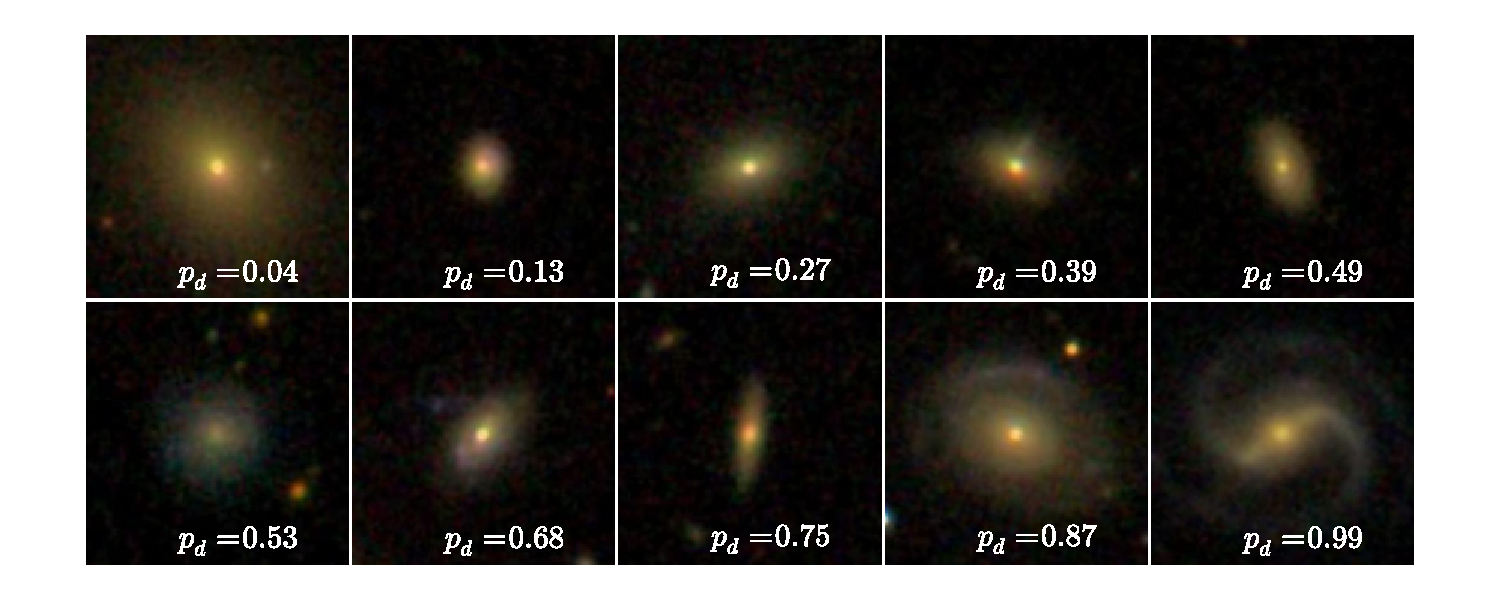
\includegraphics[width=\textwidth]{introduction/mosaic_disc_fraction_z_0-07_0-075.pdf}}
\caption[Example SDSS images with GZ2 vote fractions]{Randomly selected SDSS $gri$ composite images showing the continuous probabilistic nature of the Galaxy Zoo sample from a redshift range $0.070 < z < 0.075$. The debiased disc vote fraction for each galaxy is shown. The scale for each image is $0.099~\rm{arcsec/pixel}$.}
\label{fig:mosaic}
\end{figure}

\begin{figure}[t]
\centering{
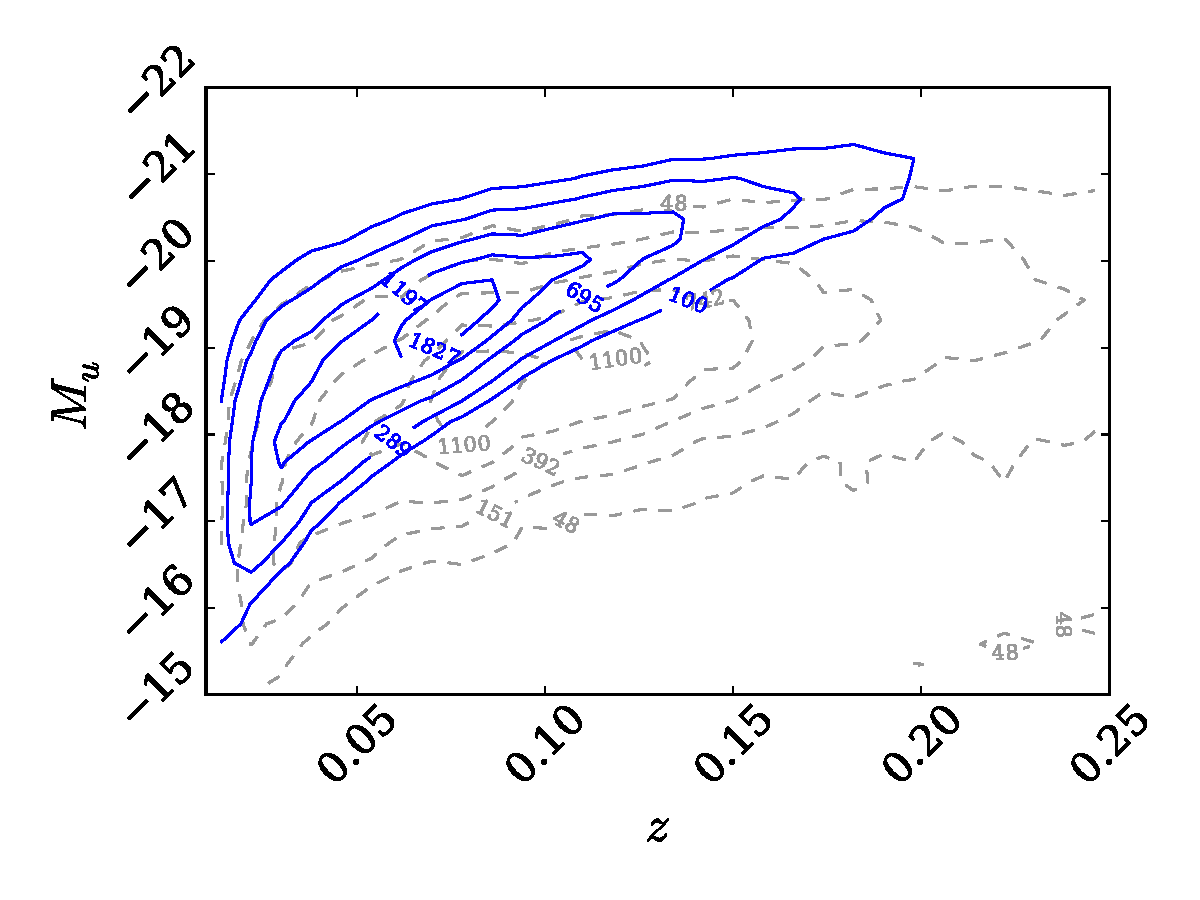
\includegraphics[width=\textwidth]{introduction/mag_redshift_completeness.pdf}}
\caption[GZ2-GALEX sample completeness]{Absolute $u$-band magnitude against redshift for the whole of SDSS (grey dashed lines) in comparison to the GZ2 subsample (blue solid lines). Typical Milky Way $L_*$ galaxies with $M_u \sim -20.5$ are still included in the GZ2 subsample out to the highest redshift.}
\label{complete}
\end{figure}


I require a sample of galaxies with optical and NUV photometry from SDSS and GALEX respectively, along with morphologies from GZ2 in order to study the morphological dependence of galaxy quenching histories. The GZ2 sample consists of $304,022$ SDSS galaxies which were selected to include the brightest ($m_r < 17$), largest (radius containing $90\%$ of the Petrosian flux, $r_{90} > 3''$) and nearest ($0.005 < z < 0.25$) galaxies in order to achieve robust detailed morphological classifications. I first removed those objects considered to be stars or artefacts in Task 0 or merging pairs in Task 6 (using the thresholds defined in Table~\ref{table:votes}) from this GZ2 sample. Further to this, I required NUV photometry from the GALEX survey, within which $\sim42\%$ of the GZ2 sample galaxies were observed, giving a total sample size of $126, 316$ galaxies. This will be referred to as the \textsc{gz2-galex} sample\footnote{No attempt is made to remove unobscured Type 1 AGN from the \textsc{gz2-galex} sample. Unobscured AGN have characteristic colours in optical imaging bands, therefore the contribution of the AGN to the galaxy photometry leads to an inaccurate estimate of the SFH. However, this effect will be negligible across the \textsc{gz2-galex} sample given the expected small fraction of unobscured AGN.}. 

The \textsc{gz2-galex} sample is shown in Figure~\ref{complete} with the $u$-band absolute magnitude against redshift, compared with the SDSS data set. Despite the GZ2 selection for the brightest and largest galaxies and the cross match to GALEX (which has a higher magnitude limit than SDSS) typical Milky Way $L_*$ galaxies with $M_u \sim -20.5$ are still included in the GZ2 subsample out to the highest redshift of $z \sim 0.25$; however dwarf and lower mass galaxies are only detected at the lowest redshifts. The redshift is taken into account during the SFH modelling (see Section~\ref{qmod}).

Galaxy colours were not corrected for intrinsic dust attenuation. This is of particular consequence for disc galaxies, where attenuation increases with increasing inclination. \cite{Buat05} found the median value of the attenuation in the GALEX NUV passband to be $\sim 1$ mag. Similarly \cite{masters10a} found a total extinction from face-on to edge-on spirals of 0.7 and 0.5 mag for the SDSS $u$ and $r$ passbands and show spirals with $\log(a/b) > 0.7$ have signs of significant dust attenuation. For the \textsc{gz2-galex} sample I find $\sim10\%x$ of discs (with $p_d > 0.5$) have $\log(a/b) > 0.7$, therefore we must be aware of possible biases in the results due to dust. Such biases will cause the SFH of a dusty galaxy to be inferred with less recent and faster quenching. 

Galaxy stellar masses are estimated using the method outlined in \cite{Baldry06}, who  fit a relationship between the observed $u-r$ colour and the $r$-band mass-to-light ratio, $(M_*/L_r)$, of a galaxy as:
\begin{equation}\label{baldrymlur}
\log(M_*/L_r) =
\begin{cases}
-0.95 + 0.56(u-r) & \text{if } (u-r) < 2.1 \\
-0.16 + 0.18(u-r) & \text{if } (u-r) \geq 2.1. 
\end{cases}
\end{equation}
The $r$-band mass-to-light ratio is calculated from the r-band absolute magnitude, $\mathcal{M}_r$, of a galaxy as outlined in \cite{blanton01}:
\begin{equation}\label{blanton}
\log(M_*/M_{\odot}) = \left(\frac{\mathcal{M}_{r,\odot} - \mathcal{M}_r}{2.5}\right) + \log\left(\frac{M_*}{L_r}\right),
\end{equation}
where $\mathcal{M}_{r,\odot}$ and $M_{\odot}$ are the $r$-band absolute magnitude and stellar mass of the Sun respectively. 

I shall use the \textsc{gz2-galex} sample to probe how different quenching mechanisms cause galaxies of different morphologies and environments to transition from the SFS to quiescence. 


\section{Thesis Summary}\label{sec:thesissum}


This thesis proceeds as follows. In Chapter~\ref{chap:starpy} I describe the SFH model used to characterise the colours of quenching galaxies, along with the statistical methods used to determine the distribution of quenching histories in a population of galaxies. In Chapter~\ref{chap:morph} I apply this method across the red sequence, green valley and blue cloud and investigate the morphological dependence of quenching histories in these populations. Chapter~\ref{chap:agn} is split into two parts. In Section~\ref{sec:agnfeedback} I investigate the effect of AGN feedback on the quenching histories of a  population of AGN host galaxies. In Section~\ref{sec:intbulgeless} I investigate the proposed slow co-evolution of galaxies with their central black holes, by measuring the black hole masses of a sample of bulgeless galaxies, which have assumed merger free histories. In Chapter~\ref{chap:env} I return to investigating the quenching histories of galaxies, this time focussing on the effect of the group environment on satellite galaxies in comparison to centrals and those in the field. In Chapter~\ref{chap:discussion} I discuss how the implications of my results in the context of galaxy evolution and propose ideas for future work.

Where necessary I adopt the Planck 2015 cosmological results \citep{planck16} with $(\Omega_m, \Omega_{\lambda}, h) = (0.309 \pm 0.006, 0.691 \pm 0.006, 0.677 \pm 0.005)$. 
